\documentclass[a4paper,10pt]{article}
\usepackage[letterpaper, top=1in, bottom=1in, inner=1in, outer=1in, columnsep=2pc, foot=.25in]{geometry}
\usepackage{graphicx}
\usepackage{url}
\usepackage{setspace}
\usepackage[small,bf]{caption}
\usepackage[compact]{titlesec}

% Macros
\newcommand{\benchmarkCommon} {definition of loader, stored procedures and benchmark coordinator }

\newcommand{\system} {Source Code Generation Tool for H-Store OLTP Benchmark }

% Now it begins
\title{\system}
\author{
        Zhe Zhang \\
        zhe@cs.brown.edu\\\\
        Department of Computer Science, Brown University
}
\date{}

\begin{document}
\maketitle

\doublespacing

%% -----------------------------------------------
%% INTRODUCTION
%% -----------------------------------------------
\section{Introduction}
H-Store~\cite{hstore} is a research OLTP DBMS project being developed in collaboration by MIT, Brown University, Yale University and HP Labs.  Based on assumptions that no long-running transaction is needed for high-end OLTP applications and OLTP DBMS can do without disks~\cite{citeulike:2326978} , H-Store has some features that do not exist in current market-leading DMBS products, for example, no multi-threading in execution engine, no locks, no redo logs and all transactions implemented in stored procedure. In order to test how well H-Store performs under various OLTP workload environments and therefore explore performance bottleneck in both physical design and system implementation, H-Store researchers have been designing benchmarks that mimic those OLTP workload environments and run the benchmarks on top of H-Store and collect statistics of performance characteristics. A laborious part of benchmark development is that, whenever a new benchmark is designed, the researcher needs to write code from scratch to implement it. The source code generation tool for H-Store OLTP Benchmark presented in this report provides a new approach of benchmark implementation under which all that needs to be done by a researcher is specifying key benchmark characteristics in a GUI. The removal of burden of writing non-benchmark-specific code saves time and makes H-Store researchers more productive and efficient in benchmark development process.
\\\\
This report is organized as followed: Section~\ref{secBenchmark} introduces high-level characteristics of OLTP benchmark and describes two benchmarks implemented by me from scratch for H-Store: TM1 benchmark and TPC-E benchmark. Section~\ref{secGenerator} demonstrates the process of generating an example benchmark using the source code generation tool and gives high-level description of how the tool is implemented . Section~\ref{secFuture} describes future work of the source code generation tool.

%% -----------------------------------------------
%% OLTP BENCHMARK
%% -----------------------------------------------
\section{OLTP Benchmark}
\label{secBenchmark}
\subsection{General characteristics}
\label{secBenchmarkGeneral}
A database benchmark is a set of computer programs that run on top of a database to evaluate its performance. Due to the fact that there are two types of databases (OLTP database and OLAP database), database benchmarks are divided into OLTP benchmarks and OLAP benchmarks correspondingly. OLTP(On-Line Transaction Processing) databases are designed to run real time business operations, whose execution unit is a transaction that can be invoked by thousands of concurrent users to insert, update and delete rows, one row at a time. OLTP benchmarks are designed to evaluate the performance of OLTP databases by measuring their \emph{OLTP throughput} that are usually expressed as the number of transactions executed per second.  OLAP(On-Line Analytical Processing) databases are designed to support super fast multi-dimensional analytical queries of read-only data from data warehouse, usually multiple rows at a time. OLAP benchmarks are designed to evaluate the performance of OLAP databases by measuring their \emph{analytical throughput}~\cite{olapBenchmark} that are usually expressed as the total processing time divided by the number of queries processed. 
\\\\
In general, the specification of an OLTP benchmark consists of a database schema, transactions, cardinality of each table, execution probability of each transaction and probability distribution of table columns and transaction parameters. The database schema specifies the structure of each table in database, including name and type of each table column, primary key, foreign keys and so on. A transaction is a set of operations(query, update, insert, delete) of tables in schema. 
\\\\
Typically, running an OLTP benchmark begins with running a data loader program that creates a database instance according to the database schema and populates each table in the database. The way of populating a table is: a number(specified in table cardinality) of rows is inserted into the table, where for each row the value of each column is generated according to integrity constraints and probability distribution. For example, for an INTEGER column that is uniformly distributed between 1 and 100000, the data loader, for each row, generates a random INTEGER uniformly selected between 1 and 100000. 
\\\\
After data loading is complete, the benchmark execution typically enters a preparation stage during which any background asynchronous tasks are complete and transactions are run against the database but results are not collected so that the database cache(if used) can warm up.   
\\\\
After its preparation stage completes, the benchmark execution enters the actual benchmark test stage during which the results of running transactions are collected. In more details, a transaction coordinator program randomly selects transactions to execute, one transaction at a time. The selection of transactions is based on transaction frequencies. Besides selecting and executing transactions, the coordinator records statistics including the amount of time it takes to execute each transaction and the number of times each transaction has been executed. It also maintains the statistics of per-transaction OLTP throughput and overall OLTP throughput. After a specified length of time elapses, the coordinator stops selecting and executing transactions and finally displays the throughput results. 
\\\\
In the next two subsections, I will describe two benchmarks that I implemented for H-Store: TM1 benchmark and TPC-E benchmark.
\subsection{TM1}
Providing relevant and objective database performance information to telecommunications providers~\cite{tm1Merlin}, TM1(Telecom One) benchmark is the first database benchmark designed for telecommunication applications~\cite{tm1Sun} and is widely used by network equipment providers as well as software and hardware vendors to compare the performance of different products~\cite{tm1Amd}. TM1 benchmark simulates a typical Home Location Register (HLR) database used by a mobile carrier, and running the benchmark shows Mean Qualified Throughput (MQTh), meaning transactions (both committed and aborted) handled per second.
\\\\
The TM1 database schema is a simplified version of a real-world HLR application schema~\cite{tm1Sun}. It stores information about subscribers, such as mobile phone numbers, current locations of subscribers' mobile devices, the services they subscribe and access privileges. There are four tables (Figure~\ref{figTm1Schema}) in the schema: Subscriber, Access\_Info, Special\_Facility and Call\_Forwarding. Typical initial cardinalities of Subscriber are: 100,000, 200,000, 500,000, 1,000,000, 2,000,000 and 5,000,000, and the initial cardinalities of Access\_Info, Special\_Facility and Call\_Forwarding are, respectively 2.5 times, 2.5 times and 3.75 times of that of Subscriber. For every column, the initial value is uniformly distributed in its value range. 
\\\\
There are seven pre-defined transactions run in TM1. 80\% of them are read transactions and 20\% are write transactions. For a given subscriber id, GET\_SUBSCRIBER\_DATA retrieves its profile; GET\_NEW\_DESTINATION retrieves its current call forwarding destination; GET\_ACCESS\_DATA retrieves its access validation data; UPDATE\_SUBSCRIBER\_DATA updates its service profile data; UPDATE\_LOCATION updates subscriber location; INSERT\_CALL\_FORWARDING adds a new call forwarding record; DELETE\_CALL\_FORWARDING removes a call forwarding record. For every transaction parameter, its value is uniformly distributed in its value range. 
\begin{figure*}
\centering
\begin{minipage}[t]{3.0in}
    \centering
    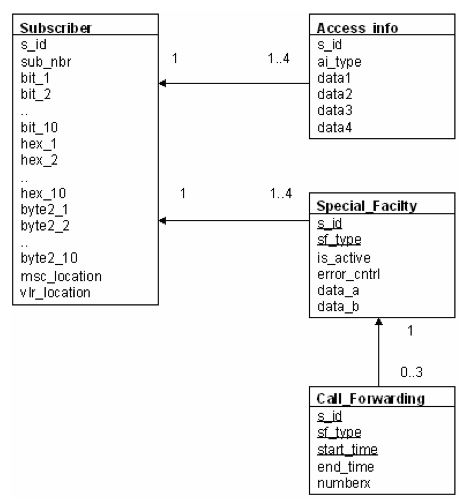
\includegraphics[width=3.0in]{img/tm1Schema.png}
    \caption{TM1 database schema~\cite{tm1Solids}}
    \label{figTm1Schema}
\end{minipage}
\end{figure*}
\\\\
Implementation of TM1 for H-Store includes TM1Loader, TM1Client (corresponding to transaction coordinator in Section~\ref{secBenchmarkGeneral}), seven stored procedures, and a schema definition file. Except from the schema definition file that comprises table-creation SQL statements, all components are written in Java and are built on top of the H-Store benchmark framework(also written in Java).  TM1Loader and TM1Client extend from class ClientMain that is the base execution class driven from standard input. Similar to the benchmark workflow mentioned in Section~\ref{secBenchmarkGeneral}, TM1Loader creates an in-memory database instance(since H-Store is an in-memory database) and populates it with generated data, and TM1Client selects transactions to execute, one at a time. Each stored procedure extends from VoltProcedure, the abstraction of a running H-Store stored procedure, and invokes SQL query methods. Maintaining and outputting of transaction throughput statistics is accomplished by the H-Store benchmark framework. 

\subsection{TPC-E}
Introduced in 2007 by Transaction Processing Performance Council, the organization that introduced the de facto industry-standard TPC-C~\cite{tpc-c} benchmark in 1992, TPC-E~\cite{tpc-e} has gradually been accepted as the new industry-standard OLTP benchmark due to its benefits over TPC-C, for example, more close to today's business model(TPC-C models a wholesale supplier while TPC-E models a brokerage house), more representative of today's schema and transaction complexity(TPC-C has 9 tables, 92 columns and 5 transactions while TPC-E has 33 tables, 188 columns and 10 transactions), and significantly lower cost of running benchmark~\cite{tpce-cost, tpcc-cost}.
\\\\
The 33 tables in TPC-E schema are divided into 4 categories: Customer-related tables, Broker-related tables, Market-related tables and Dimension-related tables. Sizing rules of tables are more complexed than TM1: while in TM1 the cardinalities of all tables are proportional to the same table, in TPC-E, for some tables, cardinalities are fixed; for some, cardinalities are proportional to CUSTOMER table; for the rest of tables, cardinalities are initially proportional to CUSTOMER table but will increase during benchmark run at a rate proportional to transaction throughput rate.
\\\\
Activities simulated in TPC-E transactions include: managers of brokerage houses generating reports on the current performance potential of various brokers; customers looking up their customer profiles and summaries of their overall standing based on current market values for all assets; customers tracking the daily trend of securities; customers conducting research on security prior to making trade-execution decisions; customers looking up the summaries of recent activities; brokerage houses processing the "ticker-tape" from the market exchange; trades looking up by customers or brokers; trades update by customers or brokers; security exchange by customers, brokers or authorized third-party; completing of stock market trades~\cite{tpce-activities}. 
\\\\
Implementation of TPC-E in H-Store is similar to TM1 in code structure, except for how the generations of data for table populating and parameters for transaction execution are implemented. While in TM1, the generation algorithms are implemented by me from scratch, in TPC-E, they are implemented in TPC-provided binary code (compiled from C++ source code), which are invoked via Java Native Interface by TPC-E loader and transaction coordinator respectively.

%% -----------------------------------------------
%% FRAMEWORK OVERVIEW
%% -----------------------------------------------
\section{\system}
\label{secGenerator}
\subsection{Motivation}
As described in Section~\ref{secBenchmarkGeneral}, common characteristics exist in code structure and execution process among all benchmarks. Nevertheless, under current benchmark implementation paradigm in H-Store, these common characteristics are not transparent to researchers. Therefore, whenever a researcher wants to implement a new H-Store benchmark, he/she has to write code to implement these common characteristics. If a researcher frequently implements new benchmarks, then implementing these common benchmark characteristics over and over again could be very painful. In one word, current benchmark implementation paradigm in H-Store impedes the productivity of researchers by forcing them to write non-benchmark-specific code in benchmark development process. 
\\\\
Researchers' productivity could be significantly enhanced if there exists a tool that could generate benchmark implementations without researchers' writing a single line of non-benchmark-specific code. This is where \system comes into play: a GUI-based tool which enables researchers to generate benchmarks by just specifying benchmark-specific data in the GUI.

\subsection{Creating an example benchmark}
\label{helloWorld}
This section goes over the process of generating an example benchmark in H-Store using the tool. In general there are three steps: 1. Set up project properties such as project name and path. 2. Specify characteristics for tables in benchmark schema 3. Specify characteristics for benchmark procedures. Detailed description of each step follows.

\subsubsection{Initial configuration}
In the initial configuration pane (see Figure~\ref{initConf}), the user needs to specify benchmark name, benchmark package name and project path. The benchmark name determines the name of transaction coordinator Java class, where the latter name will be used by the H-Store benchmark framework to perform Java runtime reflection. The benchmark package name determines the declaration of package name for all generated Java classes in the benchmark. The project path specifies where the generated Java source files are located in file system.  

\begin{figure*}
\centering
\begin{minipage}[t]{3.0in}
    \centering
    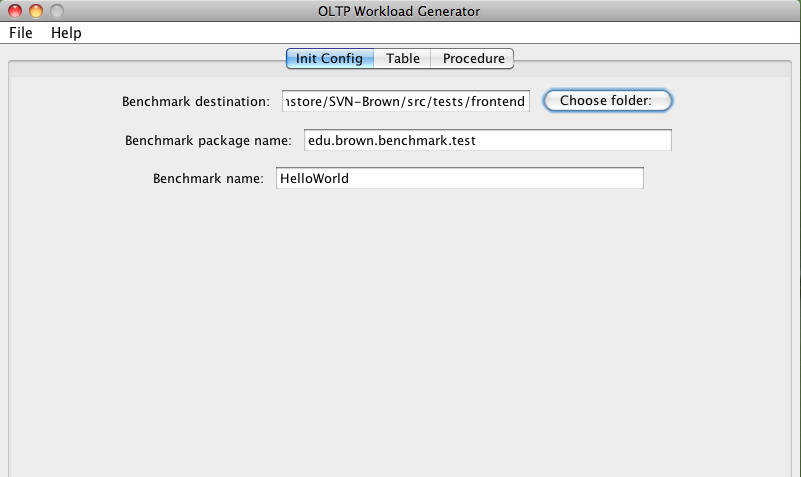
\includegraphics[width=3.0in, height=2.5in]{img/initSetup.png}
    \caption{Initial benchmark configuration}
    \label{initConf}
\end{minipage}
\begin{minipage}{0.1in}
    \hspace*{0.1in}
\end{minipage}
\begin{minipage}[t]{3.0in}
    \centering
    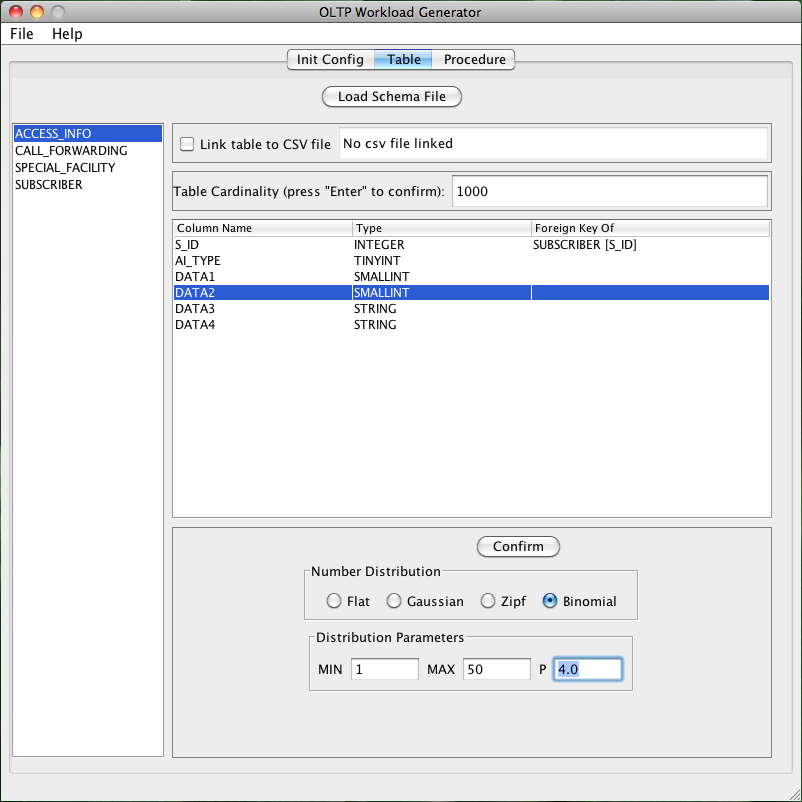
\includegraphics[width=3.0in, height=2.5in]{img/tablePane.png}
    \caption{Table configuration}
    \label{tblConf}
\end{minipage}

\end{figure*}

\subsubsection{Table configuration}
In the table configuration pane(see Figure~\ref{tblConf}), the user needs to provide adatabase schema file by clicking the \emph{Load Schema file} button. A schema file consists of table-creation SQL statements. After the schema file is chosen and parsed into its in-memory data structure, the list of table names in the schema are displayed on the left hand side of the pane. When clicking a table name in the list, the user can specify its table cardinality on the right hand side pane, which determines how many data rows will be populated into the table by Loader. Also shown on the right hand side pane are the list of columns in the table. For each column, the user needs to specify its random distribution, which determines how the value of column in each data row is generated by Loader.
\\\\
There are in total three types of column data: String, Timestamp and Number. Each data type has its own factors of random distribution. The random factor of String is its length, specified by minimum length and maximum length. The random factor of Timestamp is specified by minimum date and maximum date. The random factor of Number is its probability distribution (one of Flat distribution, Gaussian distribution, Zipfan distribution and Binomial distribution). Each distribution has its own parameters.
\\\\
Besides specifying cardinality and random distribution for columns, another way of specifying how a table is to be loaded is by linking it to a csv file (see Figure~\ref{linkCsv}) so Loader at load-time will use the data in the csv file to populate the table. Once a table is linked to csv file, the specification of table cardinality and column random factors are overriden.

\subsubsection{Procedure configuration}
In the procedure configuration pane (see  Figure~\ref{procPane}), the user needs to provide a transaction trace file by clicking the \emph{Load workload trace file} button. A workload trace file (see Figure~\ref{procTrace}) logs the information of executed procedures, such as procedure name, timestamp and execution result. H-Store infrastructure has the ability to generate such trace files when running OLTP workload. After the work load trace file is chosen and parsed into its in-memory data structure, the list of procedure names are displayed on the left hand side pane. When clicking a procedure name in the list, the user can specify its run-time execution frequency on the right hand side pane. Also shown on the right hand side pane are the list of parameters of selected procedure. For each parameter, the user needs to specify its random distribution, which determines how the value of parameter is generated when benchmark is running. Like table columns, there are three types of parameters: String, Timestamp and Number. Their random factors are the same as those of table columns.

\begin{figure*}
\centering
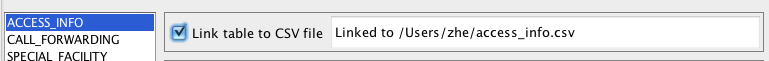
\includegraphics[width=4.0in]{img/linkCsv.png}
\caption{Link table to csv file}
\label{linkCsv}
\end{figure*}

\begin{figure*}
\centering
\begin{minipage}[t]{3.0in}
    \centering
   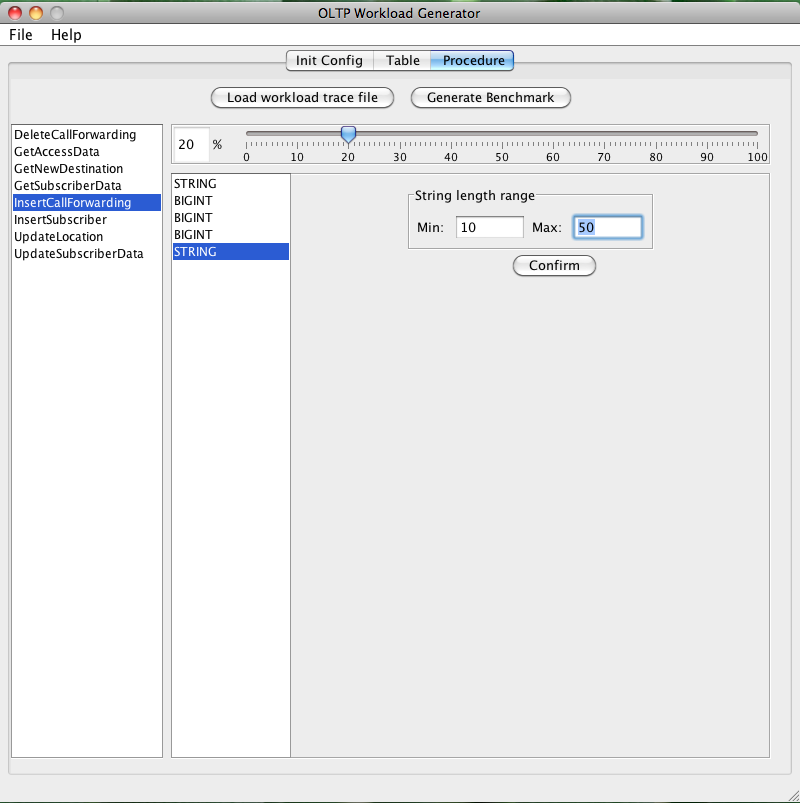
\includegraphics[width=3.0in, height=2.3in]{img/procPane.png}
   \caption{Procedure configuration}
   \label{procPane}
\end{minipage}
\begin{minipage}[t]{3.0in}
    \centering
    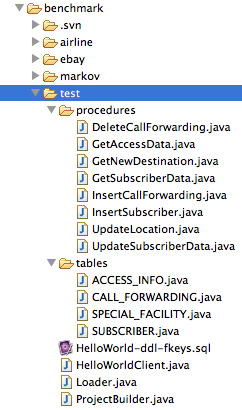
\includegraphics[width=1.5in, height=2.3in]{img/generatedBenchmark.png}
    \caption{Generated benchmark code}
    \label{generatedBenchmark}
\end{minipage}
\end{figure*}


\begin{figure*}
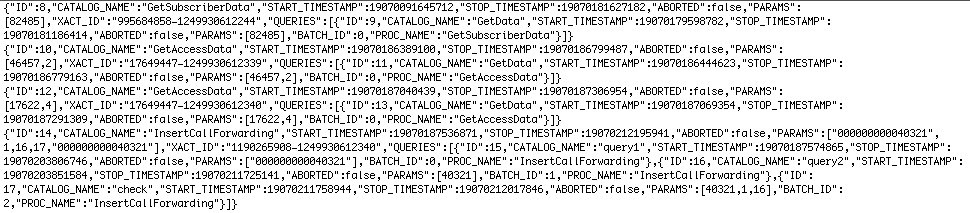
\includegraphics[scale=0.5]{img/procTrace.png}
\caption{Part of a workload trace}
\label{procTrace}
\end{figure*}

\subsubsection{Benchmark generation}
After the user specifies the initial project properties, the table characteristics and the procedure characteristics, the final step for the user is to click the \emph{Generate Benchmark} button in the procedure configuration pane. Then the benchmark implementation code will be generated and placed into destination path (see Figure~\ref{generatedBenchmark}). As can be seen from the figure, the generated implementation includes: loader(see its source code in Appendix B), transaction coordinator(which is HelloWorldClient.java), project builder(providing information to H-Store benchmark framework so that the benchmark source files can be built into class files), procedures(encoding procedure characteristics) and tables(encoding table characteristics).
\\\\
Then the user could use Volt commands(provided by the H-Store benchmark framework) to compile and run this benchmark. Retrospecting the whole benchmark implementation process, the user only needs to provide a pre-defined table schema file and a prepared workload trace file, and input benchmark characteristics in the GUI. The user doesn't need to write a single line of Java code.

\subsection{Implementation} 
The implementation of the tool is straightforward. As shown in Figure~\ref{architecture}, it is composed of a front-end module and four back-end modules: Environment, Template Engine, Templates and Abstract Benchmark. Front-end module implements the GUI on top of Java Swing/AWT API. When the user specifies the benchmark characteristics in the GUI, the characteristics get stored in Environment, which is essentially name-value pairs. When the user clicks the \emph{Generate Benchmark} button, the characteristics are read from Environment and fed to Template Engine. The Template Engine, built on top of Apache Velocity Engine(a Java-based template engine)~\cite{velocity}, binds the variables in pre-defined velocity template files to the characteristics and generates Java source files (see sample code in Appendix). Every generated source file extends from a class in Abstract Benchmark: it reuses (by invoking) its non-benchmark-specific methods such as table loading algorithm and overrides (by hardcoding into) its benchmark-specific methods such as getTableCardinality(). See in Appendix B for an example of how benchmark characteristics are hardcoded in benchmark-specific methods.

\begin{figure*}
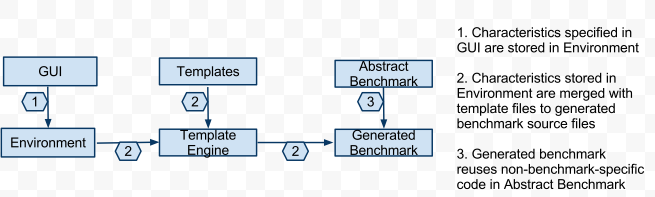
\includegraphics[scale=0.7]{img/architecture.png}
\caption{Archiecture of \system}
\label{architecture}
\end{figure*}

%% -----------------------------------------------
%% CONCLUSIONS AND FUTURE WORK
%% -----------------------------------------------
\section{Conclusions and Future Work}
\label{secFuture}
I have introduced a GUI-based source code generation tool that enables benchmark designers to implement H-Store benchmarks without needing to write Java code. More work can be done to change the fact that the user cannot save a benchmark specification to a file (and later on load it to GUI). The functionality of saving/loading benchmark specification can be useful if the user cannot complete specifying all benchmark characteristics at one time (for example, the benchmark to be implemented is too complex so the user specifies a new part in the benchmark whenever he/she has figured it out).

\bibliographystyle{abbrv}
\bibliography{FinalReport}

%% =========================================================================
%% APPENDIX
%% =========================================================================
\newpage
\appendix

%% -----------------------------------------------
%% SAMPLE SOURCE CODE
%% -----------------------------------------------
\section{Loader template file}
\begin{verbatim}
public class Loader extends AbstractLoader 
{

    private AbstractTable[] m_tables;

    public Loader(String[] args) 
    {
        super(args);
        m_tables = new AbstractTable[$tblNames.size()];
        #set( $idx = 0 )
        #foreach( $tblName in $tblNames )
          m_tables[$idx] = new $tblName();
        #set( $idx = $idx + 1 )
        #end
    }

    @Override
    protected AbstractTable[] getAllTables()
    {
        return m_tables;
    }

    public static void main(String[] args) 
    {
        org.voltdb.benchmark.ClientMain.main(Loader.class, args, true);
    }

    @Override
    protected String getSchemaFileName()
    {
        return $schemaFileName;
    }
}
\end{verbatim}

\section{Sample source code generated from Loader template file}
\begin{verbatim}
public class Loader extends AbstractLoader 
{

    private AbstractTable[] m_tables;

    public Loader(String[] args) 
    {
        super(args);
        m_tables = new AbstractTable[4];
        m_tables[0] = new SUBSCRIBER();
        m_tables[1] = new SPECIAL_FACILITY();
        m_tables[2] = new ACCESS_INFO();
        m_tables[3] = new CALL_FORWARDING();
    
    }

    @Override
    protected AbstractTable[] getAllTables()
    {
        return m_tables;
    }

    public static void main(String[] args) 
    {
        org.voltdb.benchmark.ClientMain.main(Loader.class, args, true);
    }

    @Override
    protected String getSchemaFileName()
    {
        return "HelloWorld-ddl.sql";
    }
}
\end{verbatim}

\end{document}